\documentclass[border=4pt]{standalone}
\usepackage{tikz}
\usetikzlibrary{arrows,arrows.spaced,positioning}
\begin{document}
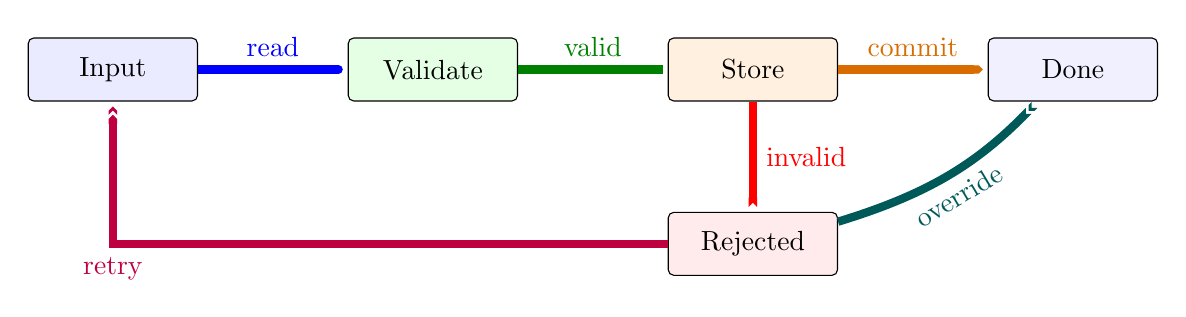
\begin{tikzpicture}[
  node distance=1.4cm and 1.9cm,
  stage/.style={draw,rounded corners=2pt,minimum width=2.15cm,minimum height=8mm,align=center}
]
  \node[stage,fill=blue!8] (input) {Input};
  \node[stage,fill=green!10,right=of input] (check) {Validate};
  \node[stage,fill=orange!12,right=of check] (save) {Store};
  \node[stage,fill=blue!6,right=of save] (done) {Done};
  \node[stage,fill=red!8,below=of save] (reject) {Rejected};

  \draw[blue,line width=3pt,-{spaced round cap}] (input) -- node[above]{read} (check);
  \draw[green!50!black,line width=3pt,-{spaced butt cap}] (check) -- node[above]{valid} (save);
  \draw[orange!85!black,line width=3pt,-{spaced triangle 90 cap}] (save) -- node[above]{commit} (done);
  \draw[red,line width=3pt,-{spaced triangle 90 cap reversed}] (save) -- node[right]{invalid} (reject);
  \draw[purple,line width=3pt,-{spaced fast cap}] (reject) -| node[below]{retry} (input);
  \draw[teal!70!black,line width=3pt,-{spaced fast cap reversed}] (reject) to[bend right=14] node[below,sloped]{override} (done);
\end{tikzpicture}
\end{document}
